\documentclass[conference]{IEEEtran}
\IEEEoverridecommandlockouts
% The preceding line is only needed to identify funding in the first footnote. If that is unneeded, please comment it out.
\usepackage{cite}
\usepackage{amsmath,amssymb,amsfonts}
\usepackage{algorithmic}
\usepackage{graphicx}
\usepackage{siunitx}
\usepackage{enumitem}
\usepackage{textcomp}
\usepackage{xcolor}
\usepackage{float}
\usepackage{listings}
\lstset{
  basicstyle=\ttfamily,
  columns=fullflexible,
  frame=none,
  breaklines=true,
  showstringspaces=false,
  postbreak=\mbox{\textcolor{red}{$\hookrightarrow$}\space},
}
\def\BibTeX{{\rm B\kern-.05em{\sc i\kern-.025em b}\kern-.08em
    T\kern-.1667em\lower.7ex\hbox{E}\kern-.125emX}}
\begin{document}

\title{EEE 145 Simulation Activity Report}

\author{\IEEEauthorblockN{Andre Mikhail Serra (X2-2)\IEEEauthorrefmark{1}, Emmanuel Jesus Estallo (X4-2)\IEEEauthorrefmark{2}, Han Espinosa(X5-1)\IEEEauthorrefmark{3}, Mark Lester Cuaresma (X4-1)\IEEEauthorrefmark{4}}
\IEEEauthorblockA{Electrical and Electronics Engineering Institute,
University of the Philippines Diliman\\
Quezon City, Philippines\\
\IEEEauthorrefmark{1}hsespinosa@up.edu.ph, 
\IEEEauthorrefmark{2}emmanuel.estallo@eee.upd.edu.ph, 
\IEEEauthorrefmark{3}andre.serra@eee.upd.edu.ph
\IEEEauthorrefmark{4}mark.lester.cuaresma@eee.upd.edu.ph
}}
\maketitle

\begin{abstract}
This paper serves as a short report on the simulation activity for the second week of EEE 145 during the midyear of AY2020-21. The report tackles the simulation of an electromechanical energy (EME) converter using MATLAB, taking into account non-ideal parameters such as the mass of the core and the sleeve damping of a typical electromagnetic solenoid setup. MATLAB's \texttt{ode45} solver is primarily used to facilitate the calculation.

\end{abstract}             

\section{Introduction}

An electromagnetic solenoid is shown below. 
\begin{centering}
\begin{figure}[h]
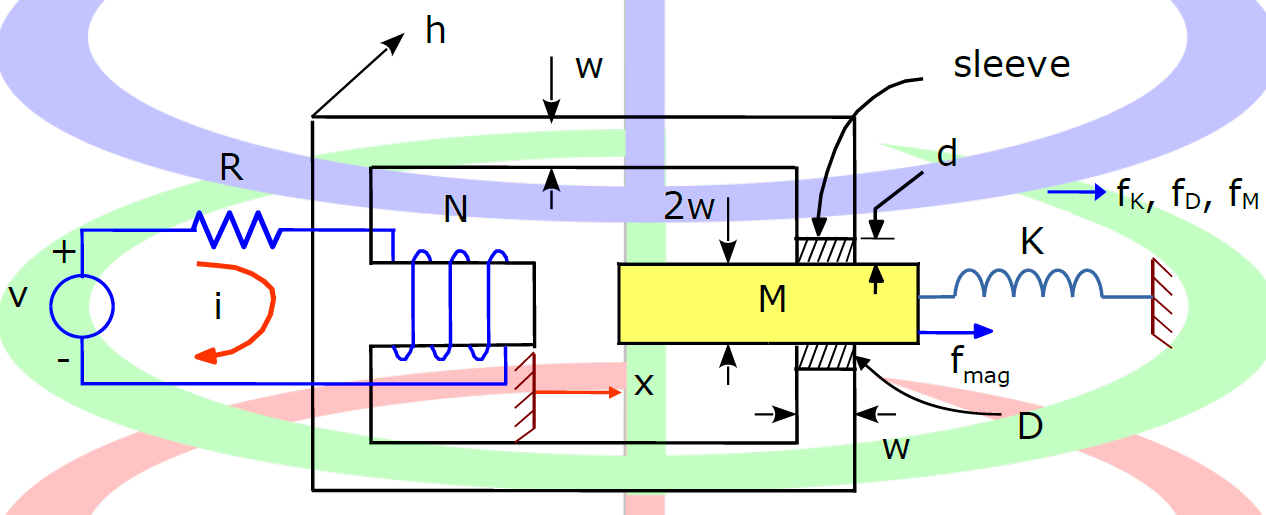
\includegraphics[scale=0.25]{solenoid.png}
\caption{Elecromagnetic Solenoid}
\end{figure}
\end{centering}

An external voltage source is connected to an $N$-winding coil wrapped around a core of some ferromagnetic material assumed to have infinite magnetic permeability. The armature of the core is fixated between two sleeves and a gap of air from the core denoted by $x$. It is also attached to a spring with a spring constant $K$, where for some $x_0$ it is unstretched.

Our task is to find an equation for the force of the magnetic field $f_{mag}$ exerted on the armature for some input current. We first go through a derivation with the assumption that the mass of the armature and of the sleeves are negligible. This is done as follows:

\begin{enumerate}
    \item Take the total reluctance of the magnetic circuit $R_{tot}$ to get the flux linkage $\lambda$;
    \item Take the derivative of the flux linkage with respect to the input current to get the inductance $L$;
    \item Find the energy or co-energy state function of the circuit using the inductance; and
    \item Take the derivative of the energy or co-energy state function to get the the force exerted by the magnetic field $f_{mag}$.
\end{enumerate}

To obtain the total reluctance, we note that the reluctance of the sleeves $R_{s}$ are in parallel to each other, and that they are in series with the reluctance of the air gap $R_{g}$. Hence, the total reluctance is simply
\begin{align*}
    R_{tot} &= R_{g} + (R_{s}|| R_{s}) \\
    &= \frac{x}{2\mu_{0} wh} + \frac{d}{2\mu_{0} wh} \\
    &= \frac{x+d}{2\mu_{0} wh}.
\end{align*}

With this, the flux linkage can be easily shown to be

\begin{equation*}
    \lambda = \frac{N^{2}i}{R_{tot}} = \frac{2\mu_{0} wh N^{2}i}{x+d}
\end{equation*}

And the inductance is thus

\begin{equation*}
    L = \frac{d\lambda}{di} = \frac{2\mu_{0} wh N^{2}}{x+d}
\end{equation*}

Note that $L$ here is independent of the current $i$. With this, we know that the co-energy state function is simply

\begin{equation*}
    W'_{fm} = \frac{1}{2} \lambda i = \frac{\mu_{0} wh N^{2}i^{2}}{x+d}
\end{equation*}

And the force is thus

\begin{equation} \label{fmag}
    f_{mag} = \frac{\partial W'_{fm}}{\partial i} = -\frac{\mu_{0} wh N^{2} i^{2}}{(x+d)^{2}}
\end{equation}

Eqn. \eqref{fmag} shown above is a result that will hold even with added complexities in our modelling of the behavior of the solenoid. 
\section{Motion and Voltage Profile}

In this activity, we use MATLAB's \texttt{ode45} solver to simulate an electromagnetic solenoid device with the following parameters: $M=\SI{20}{\gram}$; $D=\SI{0.5}{\newton\per\meter}$; $K=\SI{4.5}{\newton\per\meter}$; $d=\SI{4}{\milli\meter}$; $w=\SI{20}{\milli\meter}$; $h=\SI{40}{\milli\meter}$; $N=\SI{100}{}$; and $x_{0}=\SI{20}{\milli\meter}$, where $M$ is the mass of the armature, $D$ is the damping constant of the sleeve, $K$ is the spring constant of the plunger, $w$ and $h$ is the width and height of the core and armature, $N$ is the number of turns of the winding, and $x_{0}$ is the initial gap between the armature and the center of the core. We also assume a transition from not energized to energized.

\subsection{Ordinary Differential Equation Conversion}

When mass and damping are taken into account, two additional terms appear in the force-balance equation
for the armature; note that like $K$, the signs for $M$ and $D$ are written as such because they also tend to oppose movement in a particular direction.
\begin{equation} \label{ODE}
    -M\frac{d^{2}x}{dt^{2}} -D\frac{dx}{dt} -K(x-x_{0}) + f_{mag}=0 
\end{equation}

Eqn. \eqref{ODE} shown above is a second-order ordinary differential equation (ODE), which is not supported by the \texttt{ode45} solver. Hence, it must be converted into first order ODEs using the conversion given in the activity guide.

\begin{lstlisting}[language=matlab, numbers=left, xleftmargin=\parindent, caption=ODE function that models eqn. \eqref{ODE}]
function y_prime = calc_ode(t,y,M,D,K,a)
    mu = 1.25664e-6;
    dist = 0.004;
    w = 0.02;
    h = 0.04;
    N = 100;
    x_0 = [0.02 0];     
    y_prime = zeros(2,1);
    y_prime(1) = y(2);
    y_prime(2) = ((-mu*w*h*((N*a)^2))/((y(1)+dist)^2))/M + K*x_0(1)/M ... 
        -(D/M)*y(2) - (K/M)*y(1);  
end
\end{lstlisting}

The given function converts the second-order ODE into two first-order ODEs. It follows the conversion by introducing two new state variables $y_{1}'$ and $y_{2}'$. After taking the derivative of these state variables, we do the replacements then express only the ODE using these two state variables. Hence, it allows the \texttt{ode45} solver to work properly and accept the given parameters of the device.

\subsection{Constant Current}

In an electromagnetic solenoid, a current passing through the coils will move the armature respectively to a certain position. Using the previous function, we can now utilize the \texttt{ode45} solver and plot the position of the armature with respect to time for $0<=t<=1$. Using three different current values (\SI{0.2}{\ampere}, \SI{0.5}{\ampere}, and \SI{0.8}{\ampere}), the armature position (particularly, the gap length) with respect to time $t$ can be seen in fig. \ref{constcurrent}:

\begin{figure}
    \begin{centering}
    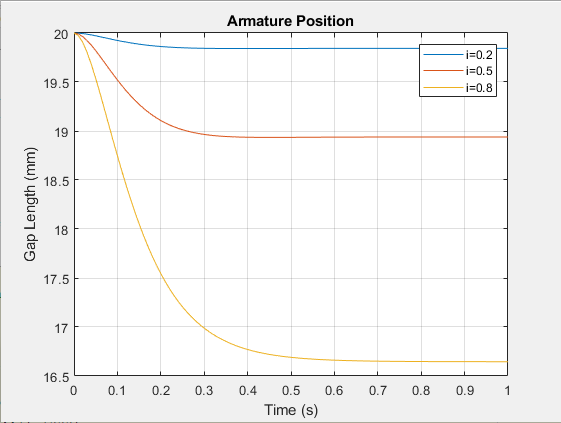
\includegraphics[width=\linewidth]{q2.png}
    \caption{Gap length vs time plot of different constant current inputs}
    \label{constcurrent}
    \end{centering}
\end{figure}

From Fig. \ref{constcurrent}, the downward slope and curvature implies the movement of the armature over time while the horizontal line is its steady state. It can be observed that when the coils have higher current, the position of the armature moves significantly longer compared to those with lower values. Specifically, at $i=\SI{0.2}{\ampere}$, the gap length is approximately \SI{19.84}{\milli\meter}, while at $i=\SI{0.5}{\ampere}$ the gap length is at \SI{18.94}{\milli\meter}. Lastly, at $i=\SI{0.8}{\ampere}$, the gap is \SI{16.65}{\milli\meter}.

Consequently, the time it takes to reach the steady state is also affected by the current passing through the coil. There is a direct relationship between the time it takes for the armature to stop moving and the value of the current. 

\subsection{Changing Current}

The behavior in the previous graph assumes that the current is constant as a function of time. However, in real systems, the current varies depending on different factors. In this problem, we assume that the current now changes with time given the equation:
\begin{equation} \label{changingcurrent}
    i(t)=c(1-exp(-30t))
\end{equation}
where $c$ is the different constant current values in the previous item.

\begin{figure}[b]
    \begin{centering}
    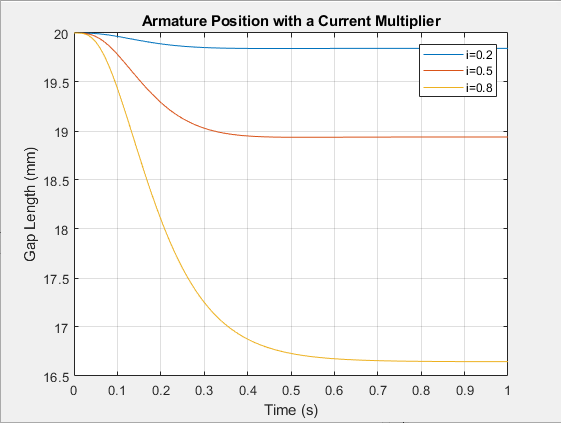
\includegraphics[width=\linewidth]{q3.png}
    \caption{Gap length vs time plot with exponentially decaying current inputs}
    \label{expcurrent}
    \end{centering}
\end{figure}

Figure \ref{expcurrent} shows the position of armature with respect to time with the current input in eqn. \eqref{changingcurrent}. The plot may seem similar to the graph of constant current since both have equal steady state values. However, it can be observed that the setup with changing current has a different rate of change compared to the those with constant current. From the current equation above, it is expected that it will reach the steady state of current at approximately \SI{0.3}{\milli\second}. Hence, the presence of degeneration in the changing current results into slower rate of change, which implies longer time to reach steady state for the armature position. Nevertheless, both setup will reach the same gap length at \SI{1}{\second}.

\subsection{Voltage Across the Coil}

This part of the activity now concerns itself with finding the voltage across the coil that induces the magnetic field. The resistances and the external voltage source are not given, so we make do with finding it by using the current input and Faraday's law for motors, as shown in eqn. \eqref{faraday} below.

\begin{equation} \label{faraday}
    \varepsilon = \frac{d\lambda}{dt}
\end{equation}

Note here that the voltage is not the negative of the change in flux because it induces the flux, and is not a reaction to the $N$-turn winding's exposure to a changing magnetic field. The following line of equations show a derivation of the expression we implement to obtain the voltage as a function of the gap length $x$.

\begin{align*}
    \varepsilon &= \frac{d\lambda}{dt} = \frac{d}{dt}\left( \frac{2\mu_{0} wh N^{2}i}{x+d} \right)= (2\mu_{0} wh N^{2}i) \frac{d}{dt} \left( \frac{1}{x+d} \right) \\
    & = (2\mu_{0} wh N^{2}i) \left( \frac{-\frac{dx}{dt}}{(x+d)^{2}} \right) = \frac{-2\mu_{0} wh N^{2}i}{(x+d)^{2}}\frac{dx}{dt} \\
    & = \frac{-2\mu_{0} wh N^{2}i}{(x+d)^{2}}x' = \frac{-2\mu_{0} wh N^{2}i}{(x+d)^{2}}y(2)
\end{align*}
The last expression makes it clear that we only need to reuse our ODE function to obtain $x'$ and get the voltage across the coil. Fig. \ref{coil1} and \ref{coil2} show the result from plotting the voltage as a function of time between the same interval as before.

\begin{figure}[b]
    \begin{centering}
    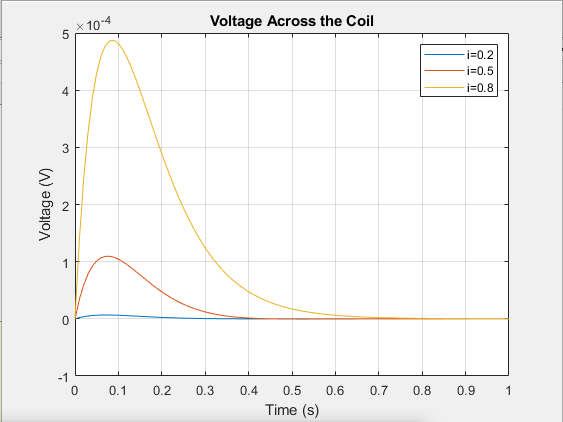
\includegraphics[width=\linewidth]{q4_1.png}
    \caption{Coil voltage vs time plot with constant current inputs}
    \label{coil1}
    \end{centering}
\end{figure}

\begin{figure}[t]
    \begin{centering}
    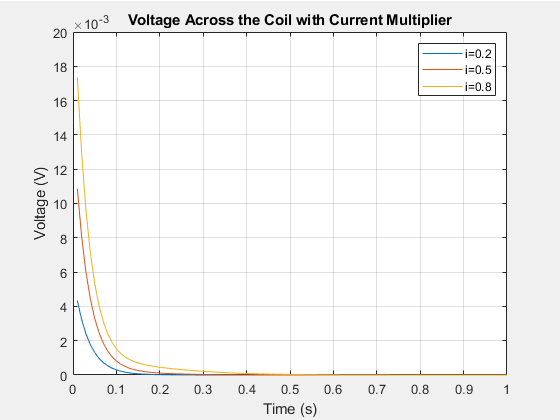
\includegraphics[width=\linewidth]{q4_2_2.png}
    \caption{Coil voltage vs time plot with exponentially decaying current inputs}
    \label{coil2}
    \end{centering}
\end{figure}

A similar derivation can be made for the exponentially-decaying current inputs, we need only take into account the derivative of the current with respect to time. Figure \ref{coil2} shows the resulting plot. There is a clear difference between the voltage's behavior across the time interval between the inputs.
\section{Appendix}
\begin{lstlisting}[language=matlab, numbers=left, xleftmargin=\parindent, caption=Full MATLAB code used in the activity]
Authors:
Mark Lester Cuaresma
Han Espinosa
Emmanuel Jesus Estallo
Andre Mikhail Serra


M = 0.02;
D = 0.5;
K = 4.5;
mu = 1.25664e-6;

%%
%question number 1
function y_prime = calc_ode(t,y,M,D,K,a)
    mu = 1.25664e-6;
    dist = 0.004;
    w = 0.02;
    h = 0.04;
    N = 100;
    x_0 = [0.02 0];
    y_prime = zeros(2,1);
    y_prime(1) = y(2);
    y_prime(2) = ((-mu*w*h*((N*a)^2))/((y(1)+dist)^2))/M + K*x_0(1)/M ... 
        -(D/M)*y(2) - (K/M)*y(1);  
end

%%
%question number 2 
i = [0.2 0.5 0.8];
t1 = 0:0.01:1;
x_0 = [0.02 0];
figure('NumberTitle', 'off', 'Name', 'Question 2');
for n = 1:3 
    [t,y] = ode45(@(t,y) calc_ode(t,y,M,D,K,i(n)), t1, x_0);
    plot(t,y(:,1)*1000)
    ylabel('Gap Length (mm)')
    xlabel('Time (s)')
    title('Armature Position')
    hold on
    grid on
    legend('i=0.2', 'i=0.5', 'i=0.8')
end

%%
%question number 3
i = [0.2 0.5 0.8];
t1 = 0:0.01:1;
x_0 = [0.02 0];
figure('NumberTitle', 'off', 'Name', 'Question 3');
for n = 1:3 
    [t,y] = ode45(@(t,y) calc_ode(t,y,M,D,K,i(n)*(1-exp(-30*t))), t1, x_0);
    plot(t,y(:,1)*1000)
    ylabel('Gap Length (mm)')
    xlabel('Time (s)')
    title('Armature Position with a Current Multiplier')
    hold on
    grid on
    legend('i=0.2', 'i=0.5', 'i=0.8')
end

%% 
%question number 4
i = [0.2 0.5 0.8];
t1 = 0:0.01:1;
x_0 = [0.02 0];
mu = 1.25664e-6;
dist = 0.004;
w = 0.02;
h = 0.04;
N = 100;
xrow = (linspace(x_0(1),x_0(2),101))'*1000;
const = ones(101,1)*(-2*mu*w*h*N*N);
figure('NumberTitle', 'off', 'Name', 'Question 4 Part 1');
for n = 1:3 
    [t,y] = ode45(@(t,y) calc_ode(t,y,M,D,K,i(n)), t1, x_0);
    plot(t, ( (const*i(n)) ./ ((y(:,1) + dist*ones(101,1)).^(2)) ) .* y(:,2))
    ylabel('Voltage (V)')
    xlabel('Time (s)')
    title('Voltage Across the Coil')
    hold on
    grid on
    legend('i=0.2', 'i=0.5', 'i=0.8')
end

%% 
%question number 4
i = [0.2 0.5 0.8];
t1 = 0:0.01:1;
x_0 = [0.02 0];
mu = 1.25664e-6;
dist = 0.004;
w = 0.02;
h = 0.04;
N = 100;
xrow = (linspace(x_0(1),x_0(2),101))'*1000;
const = ones(101,1)*(-2*mu*w*h*N*N);
figure('NumberTitle', 'off', 'Name', 'Question 4 Part 2');
for n = 1:3 
    [t,y] = ode45(@(t,y) calc_ode(t,y,M,D,K,i(n)*(1-exp(-30*t))), t1, x_0);
    emf = 2*mu*w*h*N^2*(diff(i(n)*(1-exp(-30*t))./(y+dist))./diff(t));
    plot(t(2:end),emf(:,1).*1000)
    ylabel('Voltage (V)')
    xlabel('Time (s)')
    title('Voltage Across the Coil with Current Multiplier')
    hold on
    grid on
legend('i=0.2', 'i=0.5', 'i=0.8')
end

\end{lstlisting}



\end{document}
